\section{Methods}

\subsection{Parameter Generation}
\begin{margintable}    
    \centering
    \normalsize
    \begin{tabular}{ll}
        \multicolumn{2}{l}{Optimized Parameters} \\
        \midrule
        $F_\tn{max}^\tn{ham}$              & $^{F+}G_\tn{ham}^\tn{ham}$   \\
        $F_\tn{max}^\tn{vas}$              & $^{F+}G_\tn{vas}^\tn{vas}$   \\
        $F_\tn{max}^\tn{gas}$              & $^{F+}G_\tn{gas}^\tn{gas}$   \\
        $F_\tn{max}^\tn{sol}$              & $^{F+}G_\tn{sol}^\tn{sol}$   \\
        $F_\tn{max}^\tn{ta}$               & $^{F-}G_\tn{sol}^\tn{ta}$    \\
        $^\tn{off}l_\tn{ta}^\tn{ta}$       & $^{L+}G_\tn{ta}^\tn{ta}$     \\
        $^\tn{off}\phi_\tn{knee}^\tn{vas}$ & ${^\phi}G_\tn{knee}^\tn{vas}$ \\
        $S_0^\tn{vas}$                     & $\epsilon_\tn{SE}^\tn{ap}$   \\
        $S_0^\tn{ham}$                     & $F_\tn{init}^\tn{ham}$       \\
    \end{tabular}
    \caption[Parameters optimized for parameter set generation for experiment
    comparing neuromuscular and impedance control]{Optimized parameters,
    $\Gamma$. We optimize 18 parameters. $F_\tn{max}^m$ refers to muscle $m$'s
    maximum isometric force, $S_0^m$ is muscle $m$'s pre-stimulation,
    $^\tn{signal} G_n^m$ is the gain on a feedback signal from muscle $n$
    acting on muscle $m$, $\epsilon_\tn{SE}^\tn{ap}$ is the tendon reference
    strain of the ankle plantarflexors (sol and gas) and $F_\tn{init}^\tn{ham}$
    is the initial force in the hamstring MTU at
    heelstrike.}\label{tab:nm_params_treadmill_exp}
\end{margintable}
To obtain suitable parameters for the neuromuscular and impedance control
methods we relied on the dueling bandits optimization approach outlined in
\cref{sec:bandit_optimization}. Whereas in \cref{sec:bandit_optimization} we
optimized control parameters to match gait data at different speeds to achieve a
speed-adaptive control, in this work, we optimized control parameters to match
both undisturbed and disturbed gait in order to obtain robust control
parameters. We used the dataset provided by \citet{moore2015elaborate}, which
provides gait data for undisturbed walking and walking with treadmill velocity
disturbances. 

For the neuromuscular control, we used the black-box CMA-ES optimizer
\citep{hansen2006cma} to obtain parameters that can reproduce the behavior of
each subject in the gait dataset. We optimized the parameters listed in
\cref{tab:nm_params_treadmill_exp} so the model's output torques match those in
the gait dataset. Specifically, we minimized the following cost function:
\begin{align}
    \Gamma &= \argmin_\Gamma \left(\tau_\tn{h} - \tau_\tn{nm} \right)^T
    \left(\tau_\tn{h} - \tau_\tn{nm} \right) + \alpha \xi_\tn{nm}^T \xi_\tn{nm}
\end{align}
where $\tau_\tn{nm}$ and  $\xi_\tn{nm})$ are the torques and muscle activations
respectively generated by the neuromuscular model given the human joint angle
trajectories and model parameters $\Gamma$. $\alpha = 0.01$ is a small constant
we use to help regularize the solutions and prevent muscle stimulations from
saturating. \Cref{fig:treadmill_nm_fit} shows an example of the fit achieved to
one subject's joint moments.
\begin{figure}[b]
    \centering 
    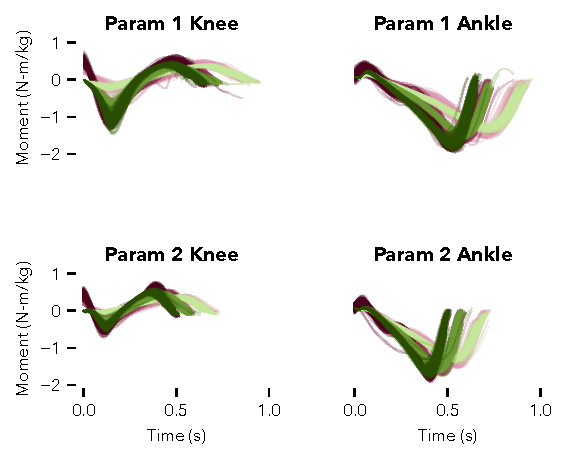
\includegraphics[width=\textwidth]{nm_fit}
    \caption{Example of fit to subject data achieved by neuromuscular
    model.}\label{fig:treadmill_nm_fit}
\end{figure}

The impedance stance control strategy we implemented, is similar to those
reviewed in \cref{sec:back_walk_fsm}. We paired this stance control strategy
with the same minimum jerk swing control as we used with neuromuscular control
(\cref{sec:nm_control_prosthesis}). \Cref{fig:impedance_control_ours} shows the
state machine for the implemented impedance stance/minimum-jerk swing control.
In each stance phase, we use a linear spring-damper relationship between the
output torque of a joint and the joint angle/velocity
(\cref{eq:impedance_func}).
\begin{marginfigure}
    \centering
    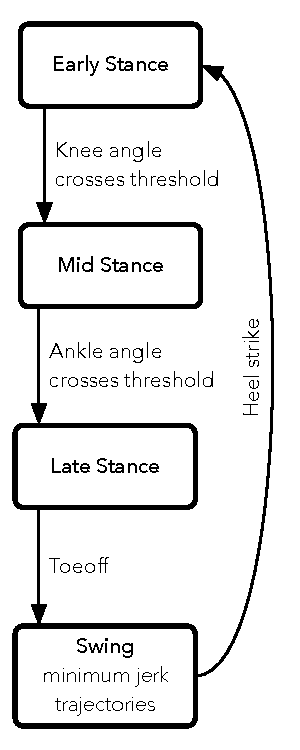
\includegraphics[width=\linewidth]{impedance_control_ours}
    \caption[Finite state machine used for impedance control scheme]{Finite
    state machine used for impedance control scheme. In each state the control
    employs linear impedance functions that determine the behavior of the ankle
    and knee joints. At toeoff, the controller generates minimum-jerk
    trajectories for the knee and ankle to follow during
    swing.}\label{fig:impedance_control_ours}
\end{marginfigure}

To generate parameters for impedance control, we followed a two step procedure:
In the first step, we identified appropriate joint angle thresholds that define
the impedance controller's finite state machine transition rules. In the
impedance controller, the transition from phase 1 to phase 2 of stance is based
on the knee angle crossing a threshold. We specified this threshold such that
95\% of steps in a subject's gait data pass from phase 1 to phase 2. As we used
gait data with disturbances, this procedure automatically sets the threshold
such that it allows for a large degree of gait variation. Next, we identified
the ankle angle threshold that defines the transition between stance phases 2
and 3.  Again, we set this threshold such that 95\% of the steps that made it
through the first transition successfully complete the second transition as
well. We set the thresholds so that 95\% of steps pass through, instead of 100\%
of steps, to ignore outlier steps.

Once we identified the joint angle thresholds that define state transitions, we
next fitted the impedance parameters within each phase. In each phase, the torque
output of the impedance control for a particular joint is 
\begin{align}
    \tau_\tn{imp} &= -k \left( \theta - \theta_0 \right) - b \dot{\theta} \\
        &= \begin{bmatrix} -\theta & -\dot{\theta} & 1 \end{bmatrix}
            \begin{bmatrix} k \\ b \\ k \theta_0 \end{bmatrix} \\
        &= \Theta \vec{k},
\end{align}
where $\Theta$ is a matrix of the subject's joint angles and velocities and
$\vec{k}$ is a vector of the impedance parameters. Therefore, the squared error
between the subject's joint torque $\tau_\tn{h}$ and the impedance control model
is
\begin{align}
    \epsilon_\tau & = {\left( \tau_\tn{imp} - \tau_\tn{h} \right)}^T 
        \left( \tau_\tn{imp} - \tau_\tn{h} \right) \\
        &= \vec{k}^T \Theta^T \Theta \vec{k} - 2\tau_\tn{h}^T \Theta \vec{k} 
        + \tau_\tn{h}^T \tau_\tn{h}.
\end{align}
To calculate the impedance parameters for each phase we minimized the squared
error subject to the constraints $k>0$ and ${b > 0}$, which ensures that the
resulting impedance models are stable. Finally, to obtain model parameters that
are robust to outlier steps in the dataset, we utilized the RANSAC procedure,
which iteratively solves the above optimization on randomly sampled subsets of
the data in order to classify outliers and fit to inliers only
\citep{fischler1981random}.

\Cref{fig:treadmill_imp_fit} shows an example of the impedance control model
optimized to match one subject's gait data. In this figure, the color of the
lines indicates the phase of gait. We see that the majority of steps fit the
subject's joint moments (grey) well. However, there are a few steps for which
the color of the line, and thus the phase does, not transition properly.
Consequently, the resulting torque diverges from the human data. This is
expected as the phase transition angles were selected such that 95\% of steps
pass through each phase transition.
\begin{figure}[t]
    \centering 
    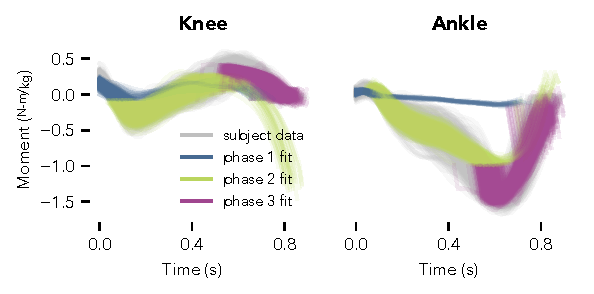
\includegraphics[width=\textwidth]{imp_fit}
    \caption[Example of fit to subject data achieved by impedance control
    model]{Example of fit to subject data achieved by impedance control model
    to. Note that green trajectories in knee moment plot and blue trajectories
    in ankle moment plot that do not track subject data are those that did not
    successfully transition to the next phase.}\label{fig:treadmill_imp_fit}
\end{figure}

\subsection{Iterative Learning}\label{sec:treadmill_exp_iterative_learning}
In~\cref{sec:bandit_methods}, in order to compensate for kinematic differences
between the joint angles in the gait dataset and the joint angles of the
prosthesis, we applied hand-tuned offsets to the measured prosthesis joint
angles before calculating the neuromuscular model torques
(\cref{eq:bias_param}). These offsets helped ensure the prosthesis achieved
comfortable levels of ankle dorsiflexion, and prevented knee over extension (or
flexion) during stance. In this experiment, in order to reduce the potential for
bias induced by hand tuning, we take a more systematic, iterative learning
approach to tuning these offsets.

During the iterative learning procedure, each subject walked with each parameter
set for both the neuromuscular and impedance controllers. The knee and ankle
angle trajectories during stance were recorded and after each step, the
following update rules were applied to the knee and ankle joint offsets
\begin{fullwidth}
\begin{align}
    \theta_\tn{knee}^\tn{offset} &\leftarrow \theta_\tn{knee}^\tn{offset} +
    k_\tn{lrn} \left(\theta_\tn{knee}^\tn{ext} - \theta_\tn{knee}^\tn{ext,tgt} \right)
    \left(\theta_\tn{knee}^\textrm{flex} < \theta_\tn{knee}^\tn{flex,max}
    \textrm{~OR~} \theta_\tn{knee}^\tn{ext} > \theta_\tn{knee}^\tn{ext,tgt}\right)\\
    \theta_\tn{ankle}^\tn{offset} &\leftarrow \theta_\tn{ankle}^\tn{offset} +
    k_\tn{lrn} \left(\theta_\tn{ankle}^\tn{flex} - \theta_\tn{ankle}^\tn{flex,tgt} \right),
\end{align}
\end{fullwidth}
where $k_\tn{lrn} = 0.05$ controls the learning rate,
$\theta_\tn{knee}^\tn{ext}$ and $\theta_\tn{knee}^\tn{ext,tgt} = 0^\circ$ are
the measured and target knee extension in mid-stance respectively and
$\theta_\tn{ankle}^\tn{flex}$ and $\theta_\tn{ankle}^\tn{flex,tgt} = 12^\circ$
are the measured and target ankle dorsiflexion in mid-stance respectively. The
conditional terms in the knee iterative learning rule prevent the knee offset
angle from inducing more knee flexion if the knee flexion in early stance,
$\theta_\tn{knee}^\textrm{flex}$, crosses a threshold
$\theta_\tn{knee}^\tn{flex,max} = 10^\circ$.

\subsection{Treadmill Disturbance}\label{sec:treadmill_exp_disturbance}
In our experiment we probed the robustness of the impedance and neuromuscular
prosthesis controllers. To this end, we disturbed gait using treadmill velocity
disturbances similar to those in the gait dataset we used to generate parameters
\citep{moore2015elaborate}. During the disturbed walking conditions, the
treadmill velocity was generated as follows: First, random accelerations were
sampled from a zero-mean Gaussian distribution with variance
$\unitfrac[35]{m^2}{s^4}$. These accelerations were saturated to the range,
$\unitfrac[{[-15, 15]}]{m}{s^2}$. Next, the acceleration was integrated to
obtain a velocity signal, and the long-term drift as removed by a $2^\tn{nd}$
order high-pass filter with a passband edge frequency of \unit[0.5]{hz}.
Finally, a constant offset of \unitfrac[0.8]{m}{s} was applied to the velocity
signal, which was then saturated to the range $\unitfrac[{[0, 3.6]}]{m}{s}$.

\subsection{Experimental Protocol}

We evaluated the robustness, user ratings, and causes for falls of the
neuromuscular and impedance controllers in an experiment with ten able-bodied
subjects wearing the prosthesis via an adaptor. All subjects provided informed
consent to IRB-approved protocols. Subjects participated in the following
six-day procedure:

\todo{also include subject stats}

\begin{days}
    \item\label{list:exp_day_1} \emph{Practice Session} Subjects practiced
    walking on the prosthesis until they could achieve consistent gait without
    the use of hand-rails. Subjects who could not achieve hands free walking by
    the end of the two-hour practice session did not continue with the
    experiment.

    \item\label{list:exp_day_2} \emph{Practice Session} On the second day
    subjects continued to practice walking on the prosthesis without the use of
    hand rails. In addition, on this day subjects practiced walking with the
    disturbance described in \cref{sec:treadmill_exp_disturbance}. This session
    lasted for 2 hours.

    \item\label{list:exp_day_3} \emph{Iterative Learning} Subjects walked with
    each of the nine parameter sets for each controller while the iterative
    learning procedure (\cref{sec:treadmill_exp_iterative_learning}) tuned the
    joint angle offsets. 

    \item\label{list:exp_day_4} \emph{Dueling Bandits Optimization} We performed
    the dueling bandits optimization procedure (\cref{sec:bandit_methods}) to
    find each subject's preferred parameters with both controllers. The order in
    which we optimized controllers was chosen randomly.

    \item\label{list:exp_day_5} \emph{Disturbance Experiment - Practice} We
    performed a practice session for the full disturbance experiment. First,
    subjects walked without the prosthesis at \unitfrac[0.8]{m}{s} for
    \unit[2]{minutes} without disturbances and then \unit[2]{minutes} with the
    treadmill velocity disturbance enabled. After completing these no-prosthesis
    trials, subjects donned the prosthesis and tested the neuromuscular and
    impedance controllers in five rounds of trials that consisted of three
    trials each. In each trial, subjects walked without disturbances for
    \unit[1]{minute} and with disturbances for \unit[1]{minute}. In each round
    of trials, the subjects tested their preferred neuromuscular and impedance
    control parameters along with a set of suboptimal parameters for one
    controller type. Odd numbered subjects tested a suboptimal neuromuscular
    parameter set, while even numbered subjects tested a suboptimal impedance
    parameter set. For the suboptimal parameter set we chose the parameter set
    that ranked $7^\tn{th}$ out of 9 in terms of cumulative Copeland score
    (defined in \cref{sec:bandit_optimization}) at the end of the dueling
    bandits tuning procedure.

    \item\label{list:exp_day_6} \emph{Disturbance Experiment - Data Collection}
    The procedure for this day was identical to that of \cref{list:exp_day_5}.
    During these trials, a Vicon motion capture system captured the motion of
    the legs. Additionally, subjects wore an IMU that measured the roll and
    pitch of the torso during walking. During trials, we recorded the number of
    falls (measured as the number of times subjects needed to use the hand rails
    or the ceiling-mounted hardness to recover balance) and the user ratings for
    both the undisturbed and disturbed conditions of each trial. 
\end{days}

We evaluated the robustness of the two control strategies primarily by looking
at the number of falls experienced by each subject in the no disturbance and
disturbance cases. As a baseline, we also compared to the no prosthesis case. As
a secondary measures of gait robustness, we also measured the variability of the
torso pitch and roll angles. The variability is measured by subtracting the
median torso angle trajectory over the strides in a condition from the
corresponding torso angle trajectories. Then the interquartile range (IQR) of
the median subtracted trajectories is used as the measure of variability.
